\documentclass[11pt,a4paper]{article}
\usepackage[T1]{fontenc}
\usepackage[left=3cm, right=3cm, top=3cm, bottom=3cm]{geometry}
\usepackage{graphicx}
\usepackage{mathtools}
\usepackage{amssymb}
\usepackage{amsthm}
\usepackage{thmtools}
\usepackage{nameref}
\usepackage{hyperref}
\usepackage{times}
\begin{document}
	SUIT Dust Filtering Mechanism
	\section{Introduction}
	Spots introduced due to contaminants and dust grains is a common phenomenon on all optical and imaging systems. These patterns could be time dependent, wavelength dependent, parameter dependent- i.e. appearing only under certain observation configurations of the instrument, or a combination of all. The nature of the dust spots could be like large blobs to small opaque spots. 
	
	In the perview of  this document, we shall refer to a certain kind of contamination signature as `dust.' The contaminant spot should be smaller than or of the order of 25 pixels in size, and the counts within the spot should be comparable to the bias value of the image, the case being no data is recorded at the locations of `dust.' This algorithm automatically looks for such regions and replaces the `dust' with values interpolated from neighboring pixels by using morphological filters.
	
	\begin{figure}
		\centering
		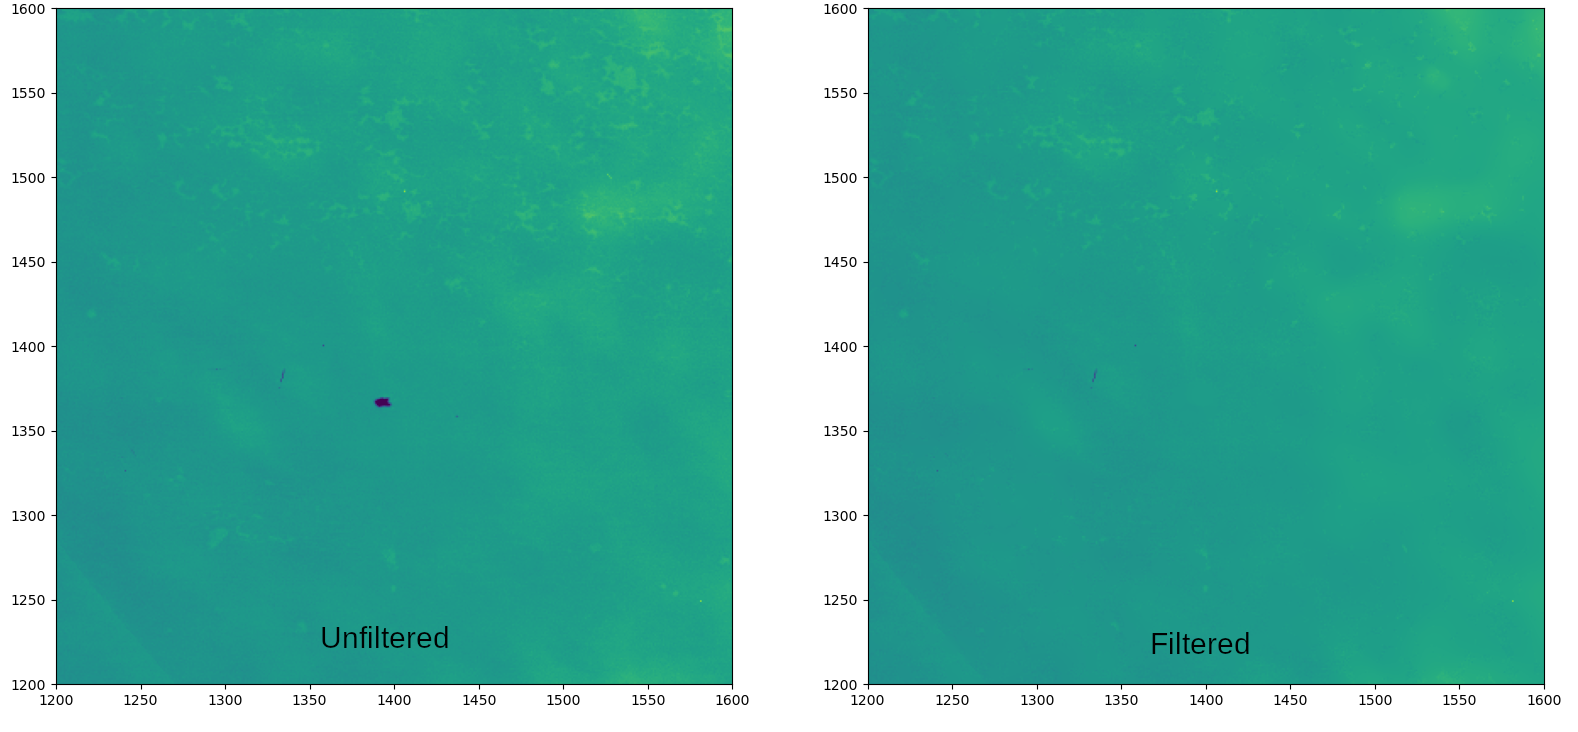
\includegraphics[width=0.7\linewidth]{pics/dust_example}
		\caption{An example of a dust spot in an image, before and after applying dust correction.}
		\label{fig:dustexample}
	\end{figure}
	
	\section{Methodology}
	\subsection{Dust Mask Method}
	\begin{itemize}
		\item SUIT LED image is used to generate a mask of all dust particles.
		\item The large scale illumination pattern of the LED images is removed using multiscale structure isolation methods, similar to that used for generating PRNU profiles for SUIT CCD.
		\item A boxcar blurring with kernel size of 4 px is applied to remove single pixel scale non uniformities.
		\item Otsu thresholding is used to create a boolean mask of the dust spots. A morphological dilation filter is applied to this mask to increase the size of the regions representing the dust spots. This is done to ensure that the mask completely occupies the dust spot.
		\item Median filtering is applied on a copy of the Sun image, with a kernel size of 10 px. The kernel size is chosen such that dust spots the are completely replaced a median value of pixels from around the dust. A smaller kernel size shall reduce the size of the dust spot instead of completely eliminating it, while a large kernel size would lead to the loss of spatial information, while also being computationally more demanding.
		\item The mask is multiplied with the median filtered image, such that the result only contains information of the masked regions.
		\item The Sun image is multiplied with the inverse of the mask, such that the dust spot regions have no data.
		\item The two resultant images are added to have an image of the Sun where the dust spots have been replaced by the median of the neighbouring pixels.
		\begin{align*}
			Resultant~image = &[Sun~image * (1-Dust~Mask) ]\\
			&+ [Median~Filtered~Sun~Image * Dust~Mask]
		\end{align*}
		\item Figure \ref{fig:dustexample} shows an example of the dust filtering.
	\end{itemize}
	\subsection{Automated dust identification and removal method}
	
	\section{Results and Conclusion}
	\begin{itemize}
		\item The Dust Mask method is effective in removing dust spots from the entire field of view. It is effective in isolating dust structures and filtering them individually. However, the dust pattern on the CCD may change with time. While the closest LED image can give us the dust pattern on the CCD, it is not representative of the dust pattern at a given date. Therefore, there can be situations where some dust spots on an image of the Sun is not corrected as well as, some regions on the Sun could be over corrected, because a dust spot is seen in the dust map but not in the Sun image.
	\end{itemize}
	
\end{document}